\documentclass{article}

\title{Assignment 3 Final Report - Electricity Discount Calculator Testing}
\date{May 10th 2020}
\author{Haioum David}

% usign math features with more convinience
\usepackage{amsmath}
%use multiple images in figures
\usepackage{subcaption}
\usepackage{graphicx}
\usepackage[export]{adjustbox}
\usepackage{caption}
% spacing
\usepackage{setspace}
% colors
\usepackage[dvipsnames]{xcolor}

%depth of the table of content
%\setcounter{tocdepth}{1} % Show sections
\setcounter{tocdepth}{2} % + subsections
%\setcounter{tocdepth}{3} % + subsubsections
%\setcounter{tocdepth}{4} % + paragraphs
%\setcounter{tocdepth}{5} % + subparagraphs

\begin{document}
    \pagenumbering{gobble}
    \maketitle
    \doublespacing
	\tableofcontents
	\singlespacing
	\newpage

    \pagenumbering{arabic} 

    \section{Test strategy}

    In this section, I will discuss on the Test strategy of the given
    electricity discount calculator code. Which means that after analyzing the software source code
    and how it works once launched, the goal is to provide the best strategy to conduct the tests.
    
    I will start by explaining my unit-testing strategy with well-known White Box testing technics. Then I will
    continue to explain how I conducted the integration tests on the main program by using black box testing technics. This
    strategy aims to follow the V-cycle model\footnote{A graphical representation of a systems development lifecycle}.

    \subsection{White box testing - Unit tests}

    We would like that every software components and functions work individually by examining each line
    of codes and its data structure. It will help to optimizing the code and determine the location of any problem. The specification
    document is given and the implementation of the code don't seem complex.

    Therefore, the chosen solution to conduct unit tests is Basic Path Testing method. The flow graphs are already given in the specification document,
    we can easily generate the flow charts to extract the cyclomatic complexity $V(G)$ and the independent paths to determine how many test cases we need to satisfy a good coverage percentage.

    By continue reading this report you will find the result of this method and whether it was effective or not.
     
    \subsection{Black box testing - Integration tests}

    For the integration test, we supose that the source code is unknown and we don't have any knowledge on the internal structure.
    This approach will be based on the legal inputs and the expected outputs of the program. 
    
    The chosen solutions are Decision Table testing and Boundary Value Analysis (BVA). The decision table is a matrix representation of the logic of a decision.
    This table is already given in the specification table and already simplified. 

    In addition, BVA complements the Decision table. We will then focus on the bundaries of the input and output values. After analyzing the specifications, we can see
    that the electricty discount calculation is based on ranges (example: comsuption is included between 0 kWh and 200 kWh). Then it is important to test the bundaries of this ranges.

    \newpage

    \section{White box testing - Unit tests}
    
    In this section let's have a closer look on the design and implementation of the unit tests

    \subsection{Test design}
    \label{section:testdesign}

    All the control flow charts have been generated by analyzing the source code and the control flow graphs from the specification document.

    \subsubsection{calcTax}

    \begin{figure}[h!]
        \includegraphics[width=0.5\linewidth, center]{cfg/calcTax.png}
        \caption{\textit{calcTax} control flow graph}
        \label{fig:cfgTax}
    \end{figure}

    \begin{equation*}
        P = 7
    \end{equation*}
    \begin{equation*}
        N = 6
    \end{equation*}
    \begin{equation*}
        V(G) = P - N + 2 = 3
    \end{equation*}
    
    \textbf{3 regions counted} and $V(G) = 3$ then \textbf{3 test cases} generated.

    \newpage

    \subsubsection{calcDiscBilNR1 and calcDiscBilNR2}

    \begin{figure}[h!]
        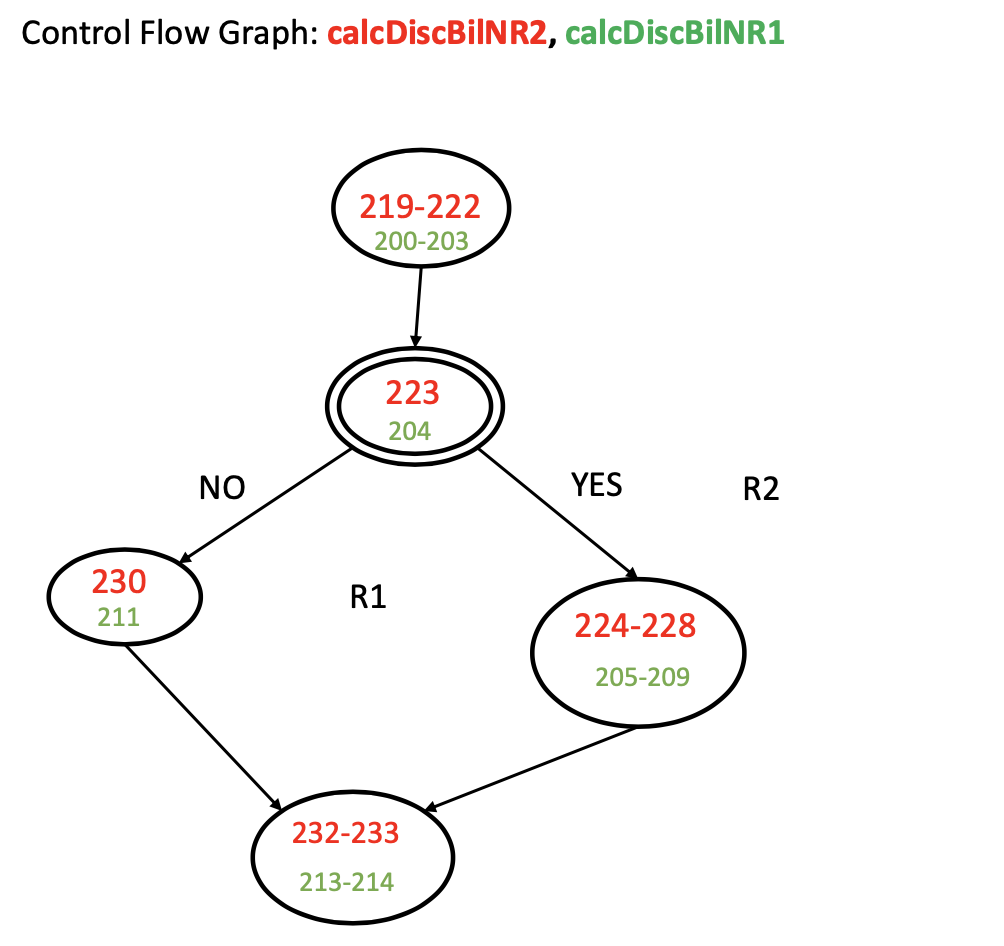
\includegraphics[width=0.5\linewidth, center]{cfg/calcDiscBilNR12.png}
        \caption{\textit{calcDiscBilNR1} and \textit{}{calcDiscBilNR2} control flow graph}
        \label{fig:cfgBilNR}
    \end{figure}

    \begin{equation*}
        P = 5
    \end{equation*}
    \begin{equation*}
        N = 5
    \end{equation*}
    \begin{equation*}
        V(G) = P - N + 2 = 2
    \end{equation*}
    
    \textbf{2 regions counted} and $V(G) = 2$ then \textbf{2 test cases} generated.

    \newpage

    \subsubsection{calcNoDiscBilNR and calcNoDiscBilR}

    \begin{figure}[h!]
        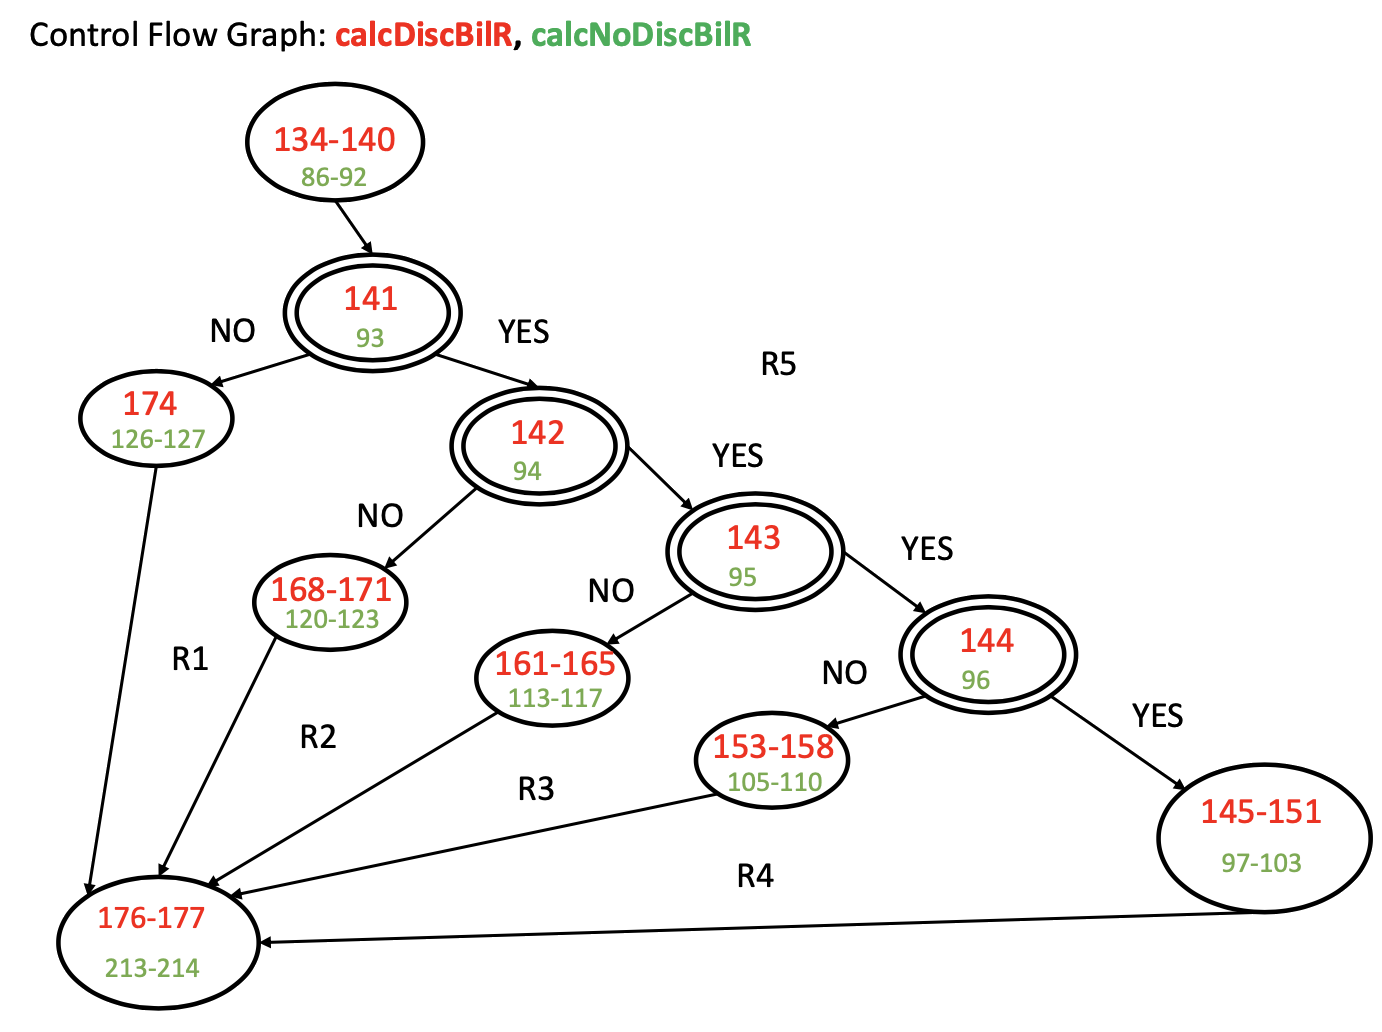
\includegraphics[width=0.6\linewidth, center]{cfg/calcDiscBilR.png}
        \caption{\textit{calcNoDiscBilNR} and \textit{}{calcNoDiscBilR} control flow graph}
        \label{fig:cfgBilR}
    \end{figure}

    \begin{equation*}
        P = 14
    \end{equation*}
    \begin{equation*}
        N = 11
    \end{equation*}
    \begin{equation*}
        V(G) = P - N + 2 = 5
    \end{equation*}
    
    \textbf{5 regions counted} and $V(G) = 5$ then \textbf{5 test cases} generated.


    \newpage

    \subsection{Test Script}

    Let's generate the test cases from the control flow charts in the section \ref{section:testdesign}.
    
    \subsubsection{calcTax function}

    \begin{figure}[h!]
        \includegraphics[width=0.8\linewidth, center]{unit_tests/calcTax.png}
        \caption{\textit{calcTax} function test cases}
        \label{fig:calcTax}
    \end{figure}
    
    \subsubsection{calcDiscBilNR1 function}

    \begin{figure}[h!]
        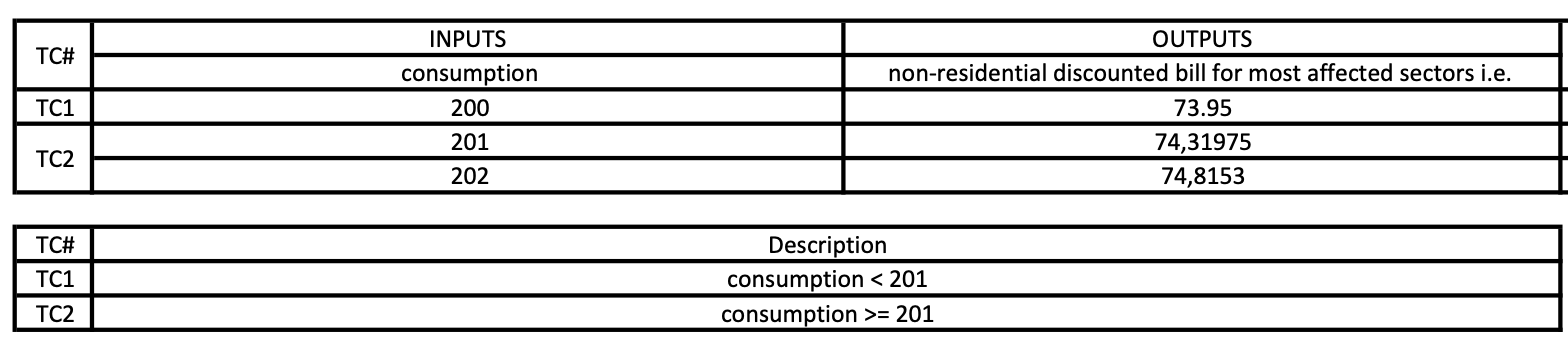
\includegraphics[width=0.8\linewidth, center]{unit_tests/calcDiscBilNR1.png}
        \caption{\textit{calcDiscBilNR1} function test cases}
        \label{fig:calcDiscBilNR1}
    \end{figure}

    \subsubsection{calcDiscBilNR2 function}

    \begin{figure}[h!]
        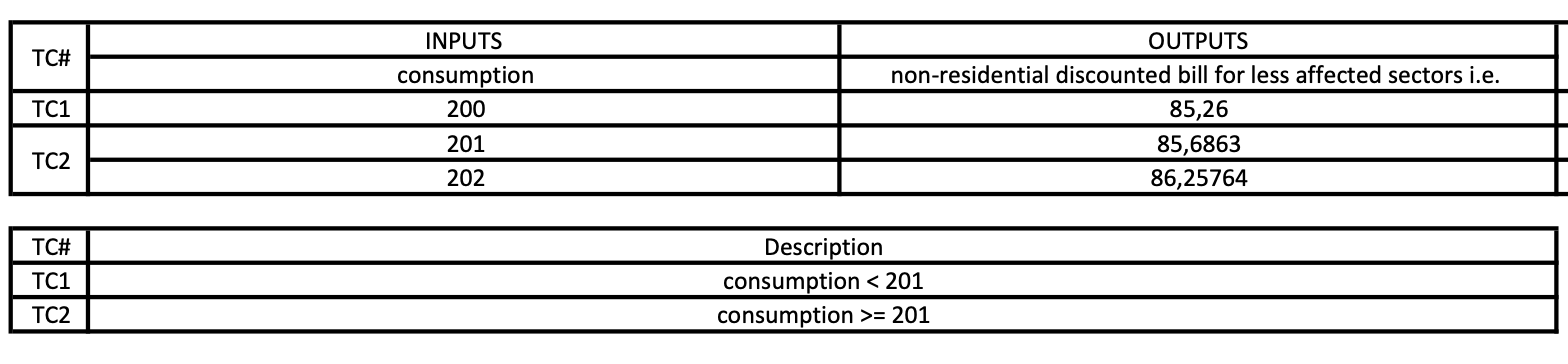
\includegraphics[width=0.8\linewidth, center]{unit_tests/calcDiscBilNR2.png}
        \caption{\textit{calcDiscBilNR2} function test cases}
        \label{fig:calcDiscBilNR2}
    \end{figure}

    \newpage

    \subsubsection{calcDiscBilR function}

    \begin{figure}[h!]
        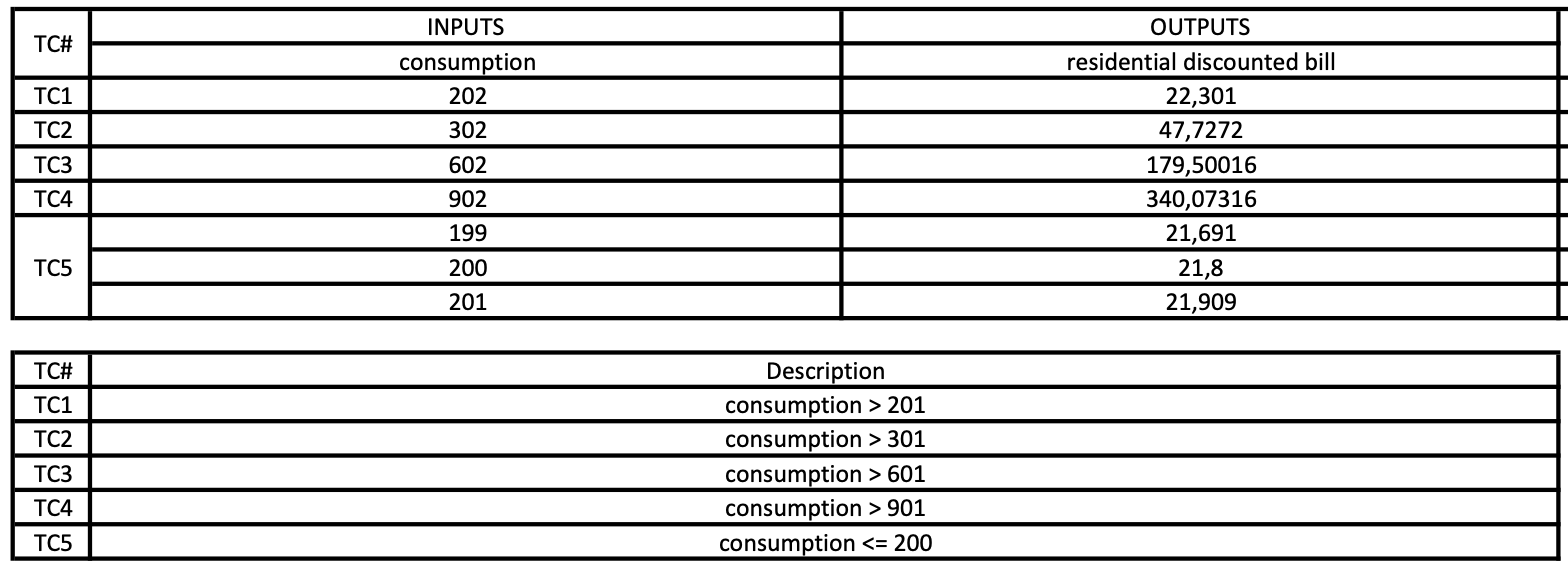
\includegraphics[width=0.8\linewidth, center]{unit_tests/calcDiscBilR.png}
        \caption{\textit{calcDiscBilR} function test cases}
        \label{fig:calcDiscBilR}
    \end{figure}

    \subsubsection{calcNoDiscBilR function}

    \begin{figure}[h!]
        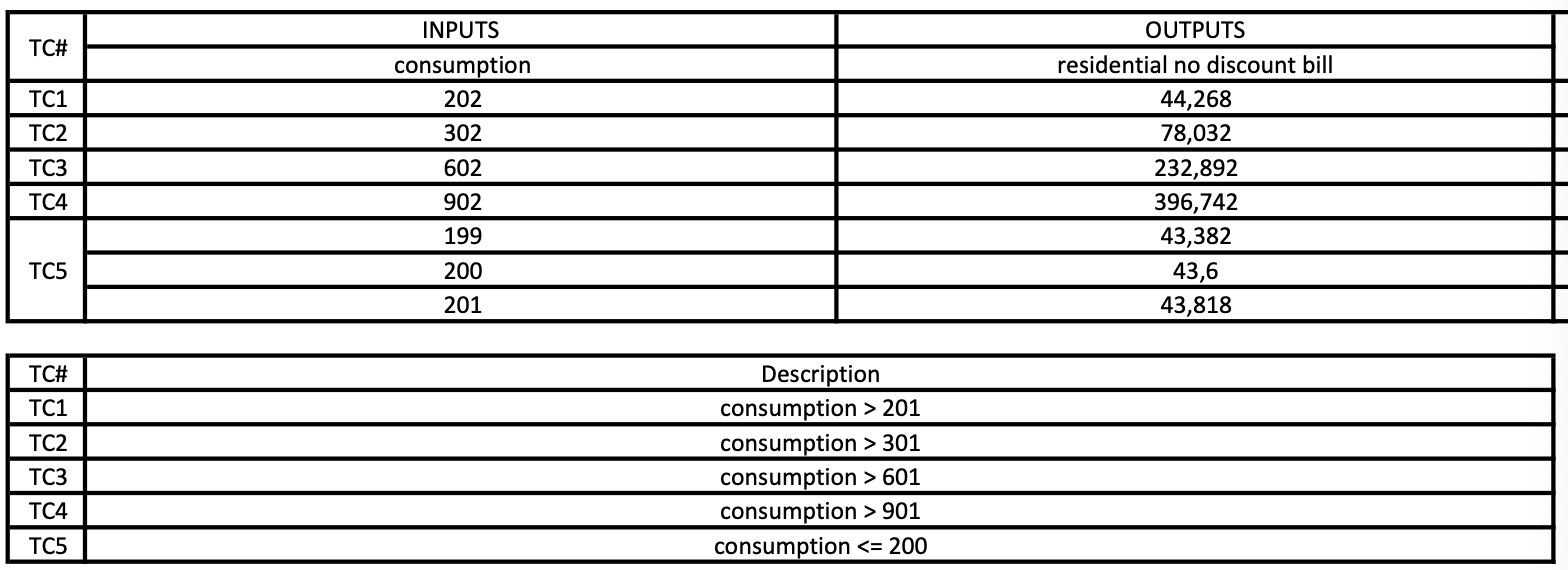
\includegraphics[width=0.8\linewidth, center]{unit_tests/calcNoDiscBilR.png}
        \caption{\textit{calcNoDiscBilR} function test cases}
        \label{fig:calcNoDiscBilR}
    \end{figure}


    \subsubsection{calcNoDiscBilNR function}

    \begin{figure}[h!]
        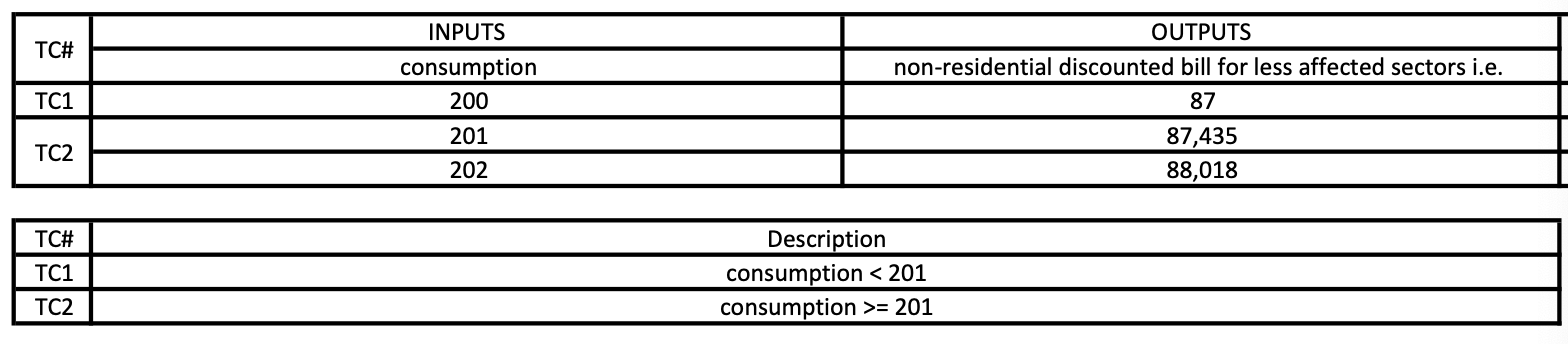
\includegraphics[width=0.8\linewidth, center]{unit_tests/calcNoDiscBilNR.png}
        \caption{\textit{calcNoDiscBilNR} function test cases}
        \label{fig:calcNoDiscBilNR}
    \end{figure}
    
    For more details, see the \underline{\textbf{\textit{unit\_tests\_cfg.pdf}}}
    document which give you the inputs and outputs of each test cases concerning unit tests only.

    \subsection{Test class (Java implementation)}

    You can see the code in the file \underline{\textbf{\textit{ElectricityDiscountCalcTest.java}}}

    \newpage

    \section{Black box testing - Integration tests}

    \subsection{Test design}
    \label{section:testdesignblack}

    The test script has been generated from the given decision table and simplified. 

    The first idea was to generate all the test cases from the given decision table. But I realized the output
    of the program was not the same. In the final test script we want to test the 7 outputs displayed in the terminal from the
    the 4 inputs provided by the user.

    We consider that the input \textit{continue} is always 0 to perform only one time the program for each test case.
    Then in the final test script, I simplified the last cases for \textit{Hotel}, \textit{Travel}, \textit{Commercial}, \textit{Industrial}.
    We will see later that this optimisation have an effect on the coverage (Figure  ~\ref{fig:newcoveragereport}). 

    \subsection{Test Script}

    For more details, see the \underline{\textbf{\textit{integration\_tests\_script.pdf}}}
    document which give you the inputs and outputs of each test cases concerning unit tests only.

    \subsection{Test class (Java implementation)}

    You can see the code in the file \underline{\textbf{\textit{ElectricityDiscountCalcIT.java}}} which is
    nested in \underline{\textbf{\textit{ElectricityDiscountCalcTest.java}}}.

    \newpage
   
    \section{Coverage information}

    \subsection{Coverage report}

    This section present you the results (Figure ~\ref{fig:coveragereport}) of the tests known as coverage that give the percentages. 
    Figure ~\ref{fig:instructioncoverageclass} illustrate why certain coverage percentages are not at 100\%. This coverage report has been made 
    on the test script with simplifications mentioned in Section \ref{section:testdesignblack}

    \begin{figure}[h!]
		\centering
		\begin{subfigure}[b]{0.4\linewidth}
			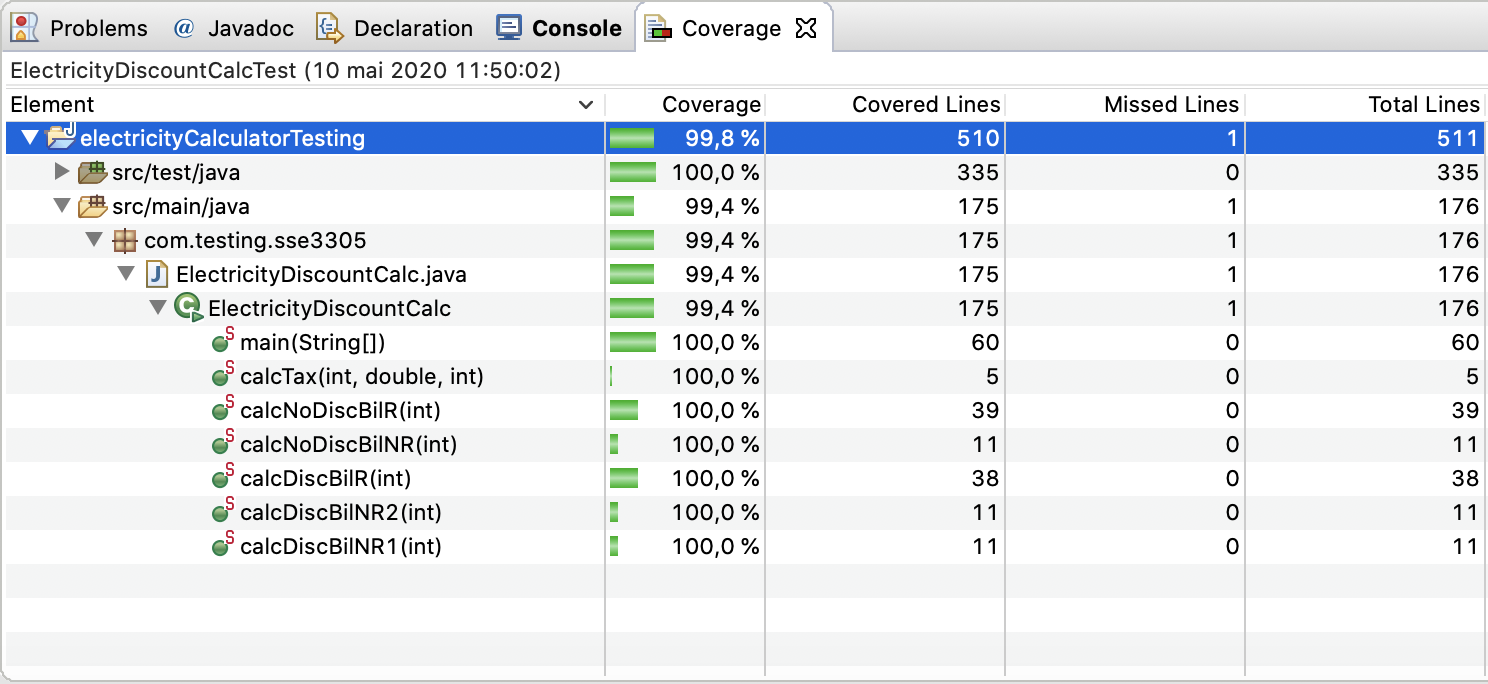
\includegraphics[width=\linewidth]{coverage/line_coverage.png}
			\caption{Line coverage}
		\end{subfigure}
		\begin{subfigure}[b]{0.4\linewidth}
			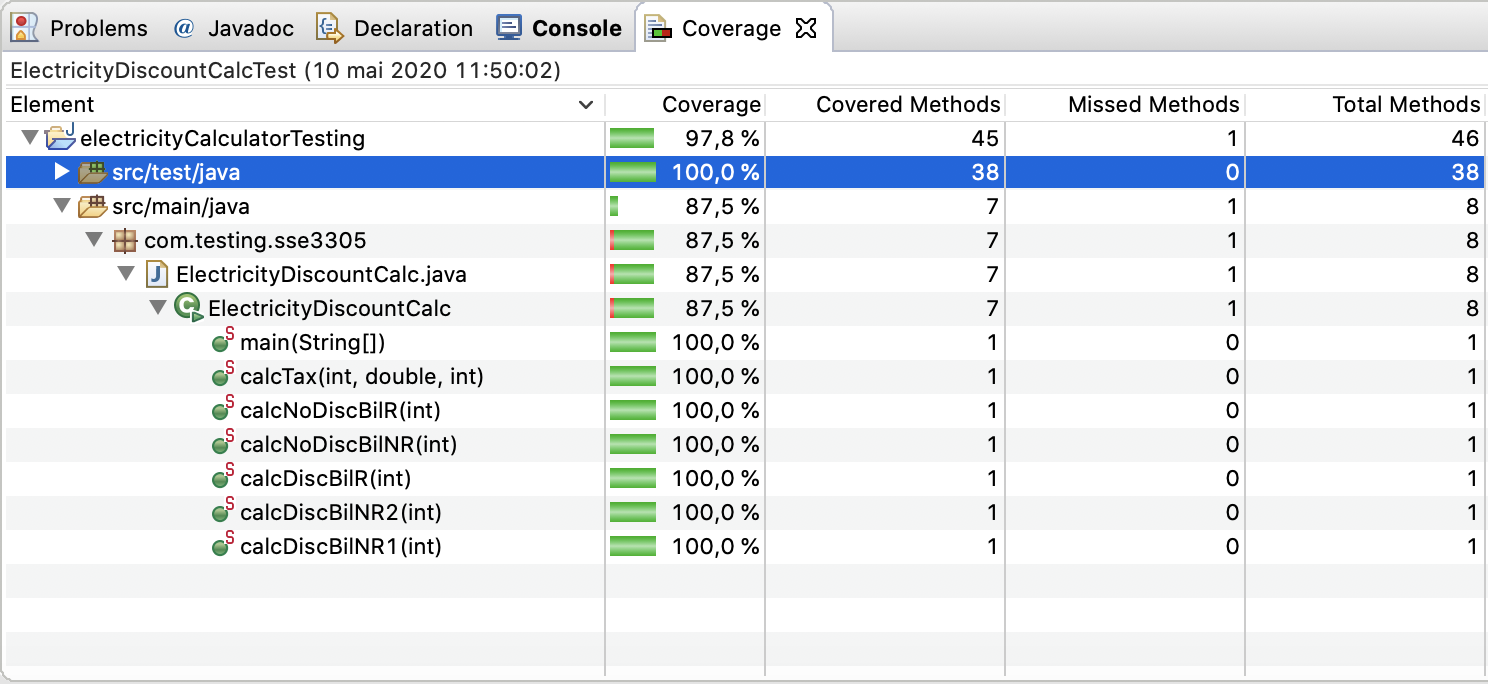
\includegraphics[width=\linewidth]{coverage/method_coverage.png}
			\caption{Method coverage}
        \end{subfigure}
        \begin{subfigure}[b]{0.4\linewidth}
			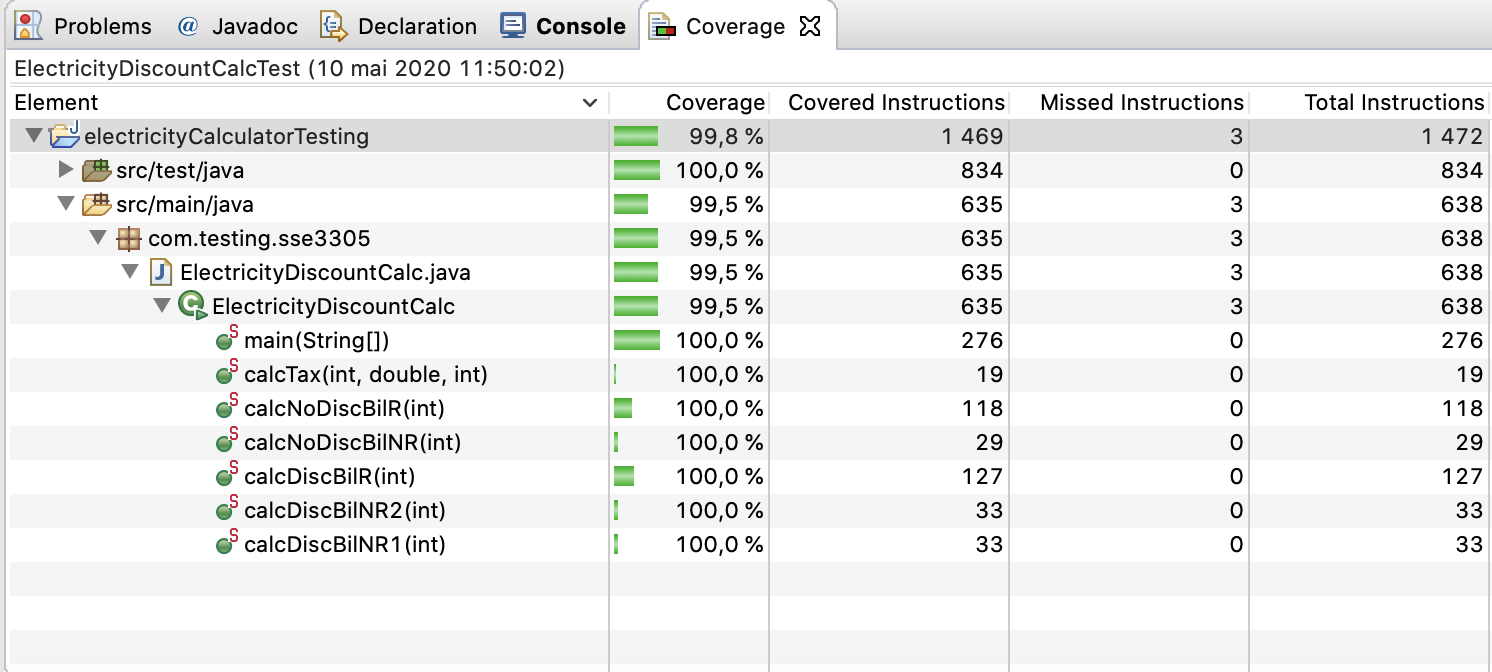
\includegraphics[width=\linewidth]{coverage/instruction_coverage.png}
			\caption{Instruction coverage}
        \end{subfigure}
        \begin{subfigure}[b]{0.4\linewidth}
			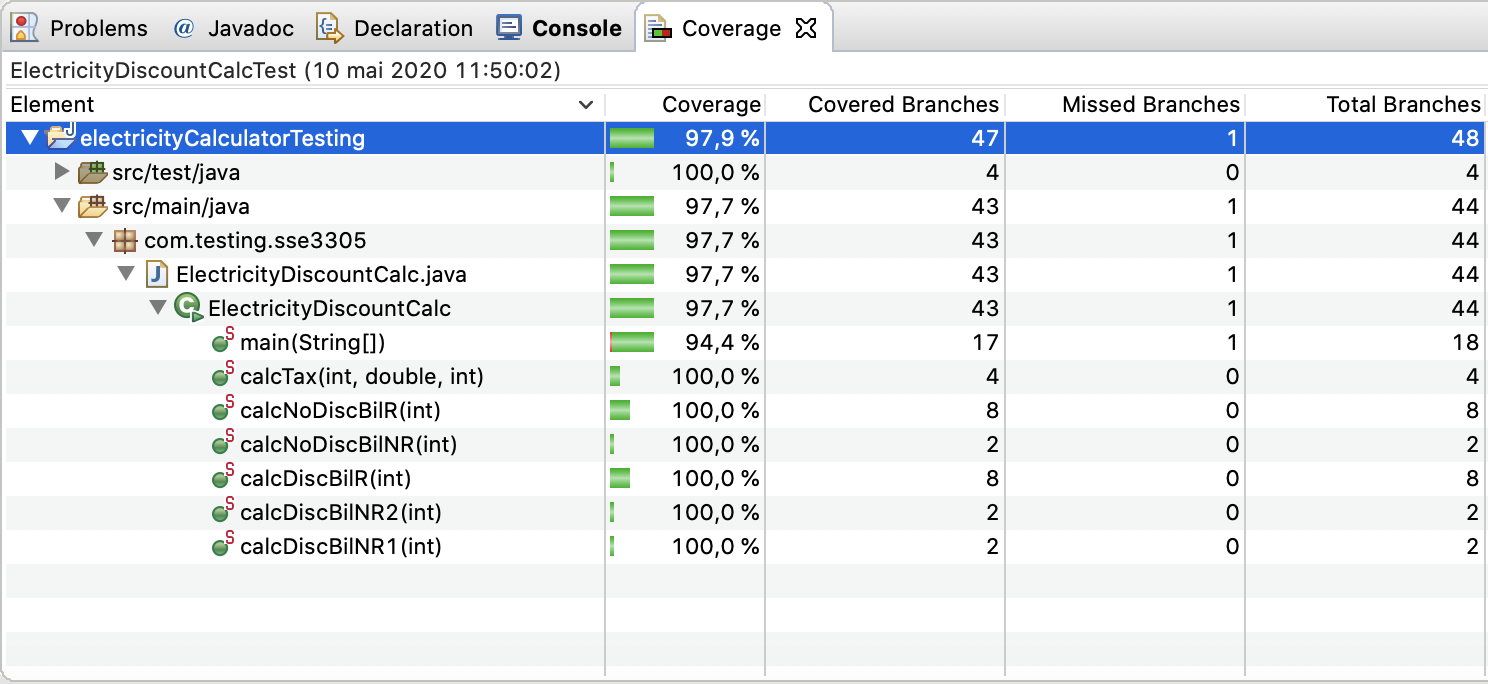
\includegraphics[width=\linewidth]{coverage/branch_coverage.png}
			\caption{Branch coverage}
		\end{subfigure}
		\caption{Test coverage report from Jacoco Eclipse}
		\label{fig:coveragereport}
	\end{figure}

    On Figure ~\ref{fig:coveragereport} - (c), we can see that the tests provide a 100\% coverage on every functions. Which means our
    tests are efficient in term of Instruction coverage (all instructions has been tested). 
    
    For line coverage (Figure ~\ref{fig:coveragereport} - (a)) as well: The tests sucessfully
    cover all the lines of code.

    However we can see that the Method coverage (Figure ~\ref{fig:coveragereport} - (b) and Branch coverage (Figure ~\ref{fig:coveragereport} - (d))
    are not completely done.  Note that even if we said that line coverage provide a 100\% coverage we can notice that the total coverage is 99.4\%.
    On the Figure ~\ref{fig:instructioncoverageclass} we can have a look on what is really happening and try to find a suitable solution.
   
    \newpage

    \begin{figure}[t!]
		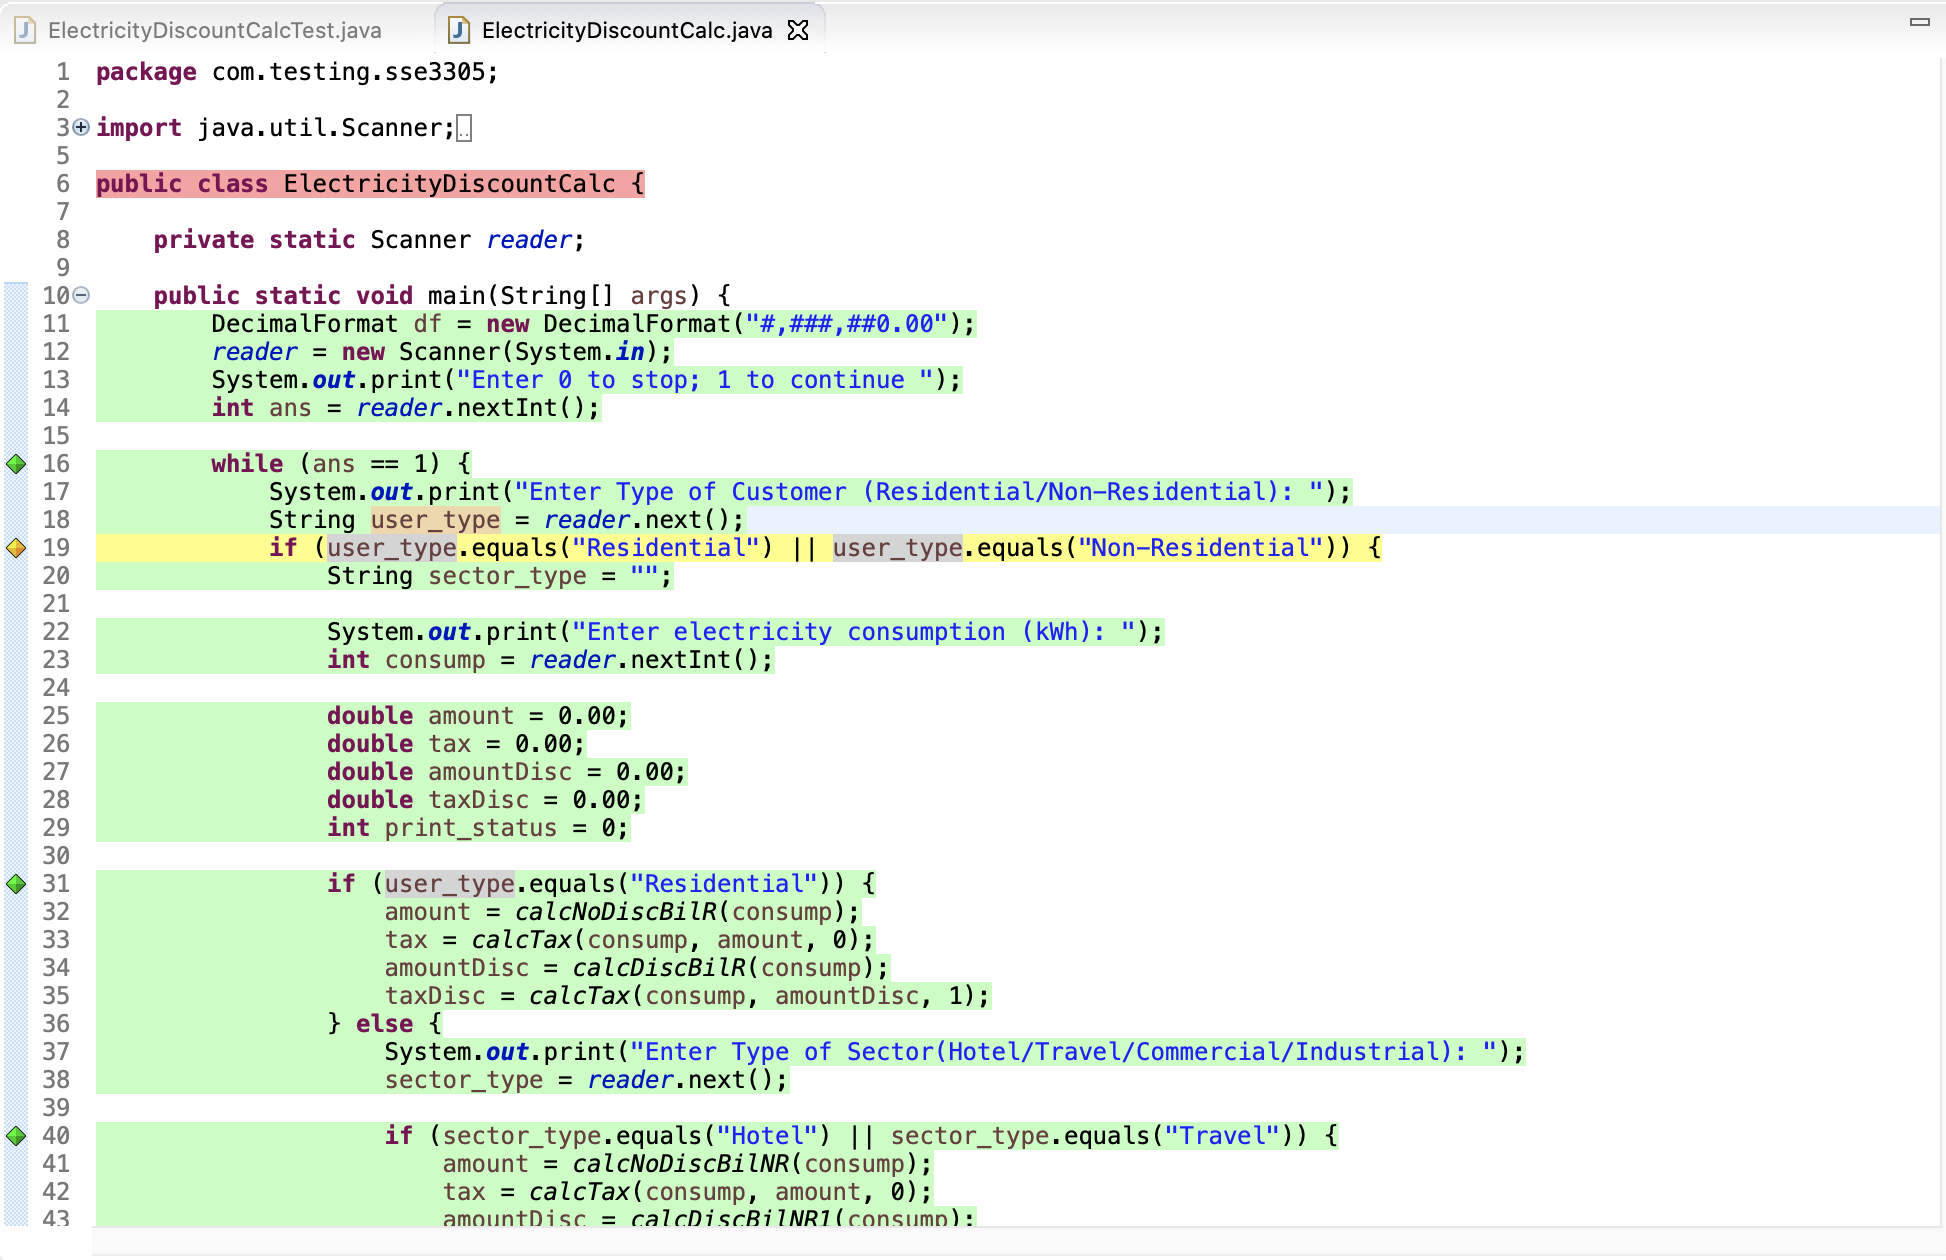
\includegraphics[width=0.8\linewidth, center]{coverage/instruction_coverage_class.png}
		\caption{The coverage of the ElectricityDiscountCalc java class}
		\label{fig:instructioncoverageclass}
	\end{figure}

    On Figure ~\ref{fig:instructioncoverageclass} at line 6 of the program, The instanciation of the class is not really tested.
    This impact the coverage percentage. We could not have predict this case in our test design. 
    So let's write a test that test the instanciation in java (Figure ~\ref{fig:instanciationtest}).

    \begin{figure}[h!]
		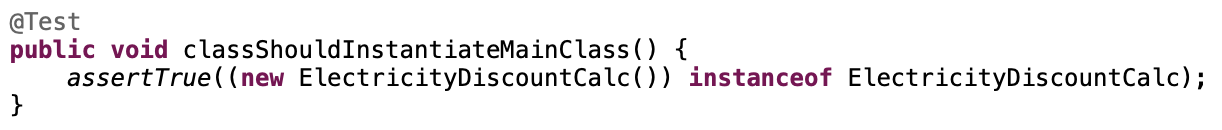
\includegraphics[width=0.8\linewidth, center]{coverage/instanciation_test.png}
		\caption{Verify the instance of ElectricityDiscountCalc java class }
		\label{fig:instanciationtest}
    \end{figure}
    
    Now we can launch again the coverage on eclipse and observe the results.

    \begin{figure}[h!]
		\centering
		\begin{subfigure}[b]{0.5\linewidth}
			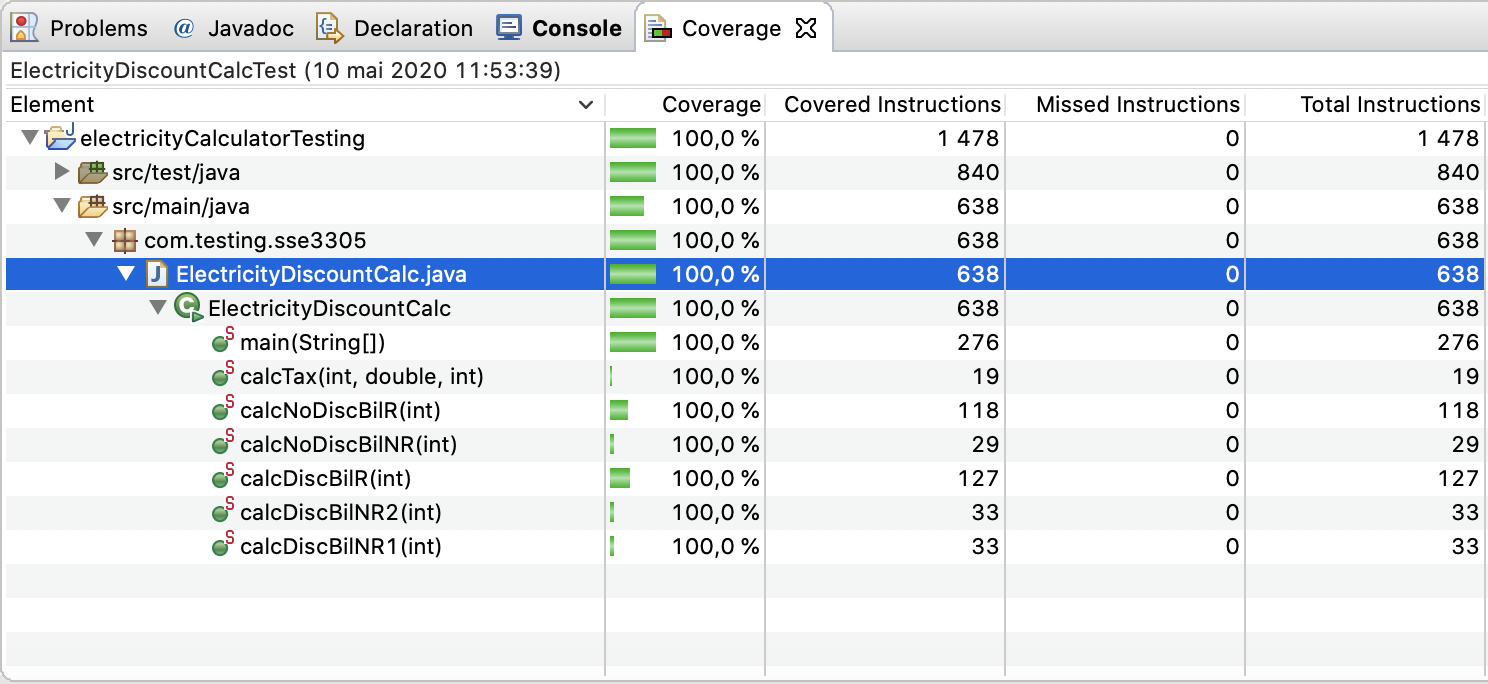
\includegraphics[width=\linewidth]{coverage/instruction_coverage_instance.png}
			\caption{Instruction coverage}
		\end{subfigure}
		\begin{subfigure}[b]{0.5\linewidth}
			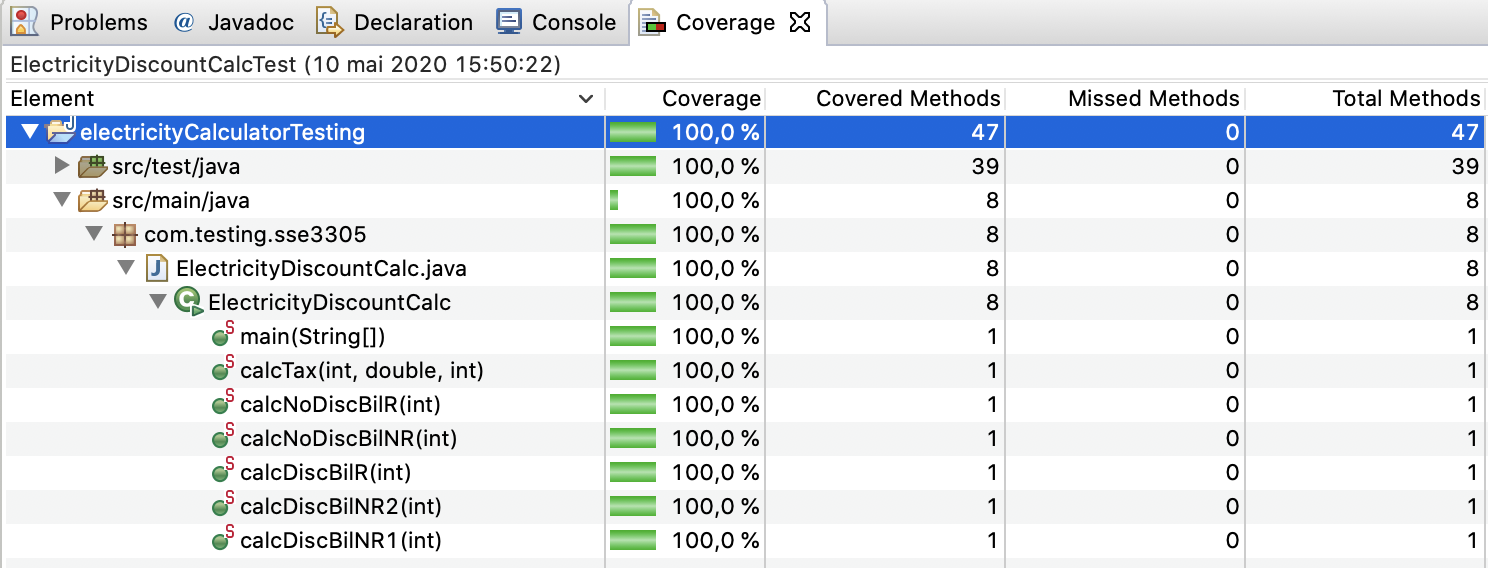
\includegraphics[width=\linewidth]{coverage/method_coverage_instance.png}
			\caption{Method coverage}
        \end{subfigure}
		\label{fig:coveragereportinstance}
    \end{figure}
    
    There is still one line (line 19 on Figure ~\ref{fig:instructioncoverageclass}) that is underline in \colorbox{yellow}{yellow} by Eclipse.
    This branch is not 100\% covered by our tests. In fact some path are not tested by our tests concerning this branch.
    The solution might be to use Control Structure Testing which is a white-box testing technique where test cases are
    generated based on the coverage of instructions of code. Of course we should avoid duplicating test cases by adding this technic.
    
    \subsection{Coverage optimisation}

    Like mentioned in Section \ref{section:testdesignblack} we would like to know if the optimisation made in the decision table can have any impact
    on the coverage percentage. At first we could say yes. We expect the coverage to be higher.

    \bigskip

    Let's now implement the new test cases

    \begin{figure}[h!]
		\centering
		\begin{subfigure}[b]{0.3\linewidth}
			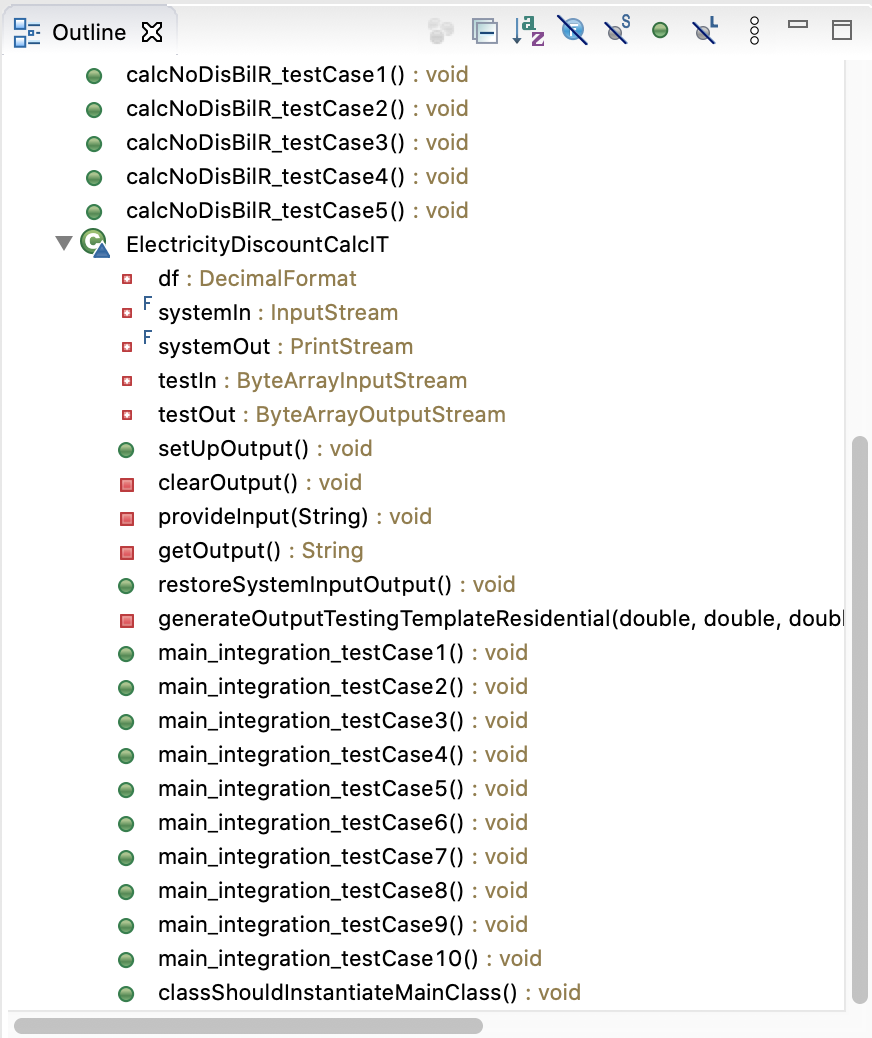
\includegraphics[width=\linewidth]{coverage/opti/10testcases.png}
			\caption{Original test script}
		\end{subfigure}
		\begin{subfigure}[b]{0.3\linewidth}
			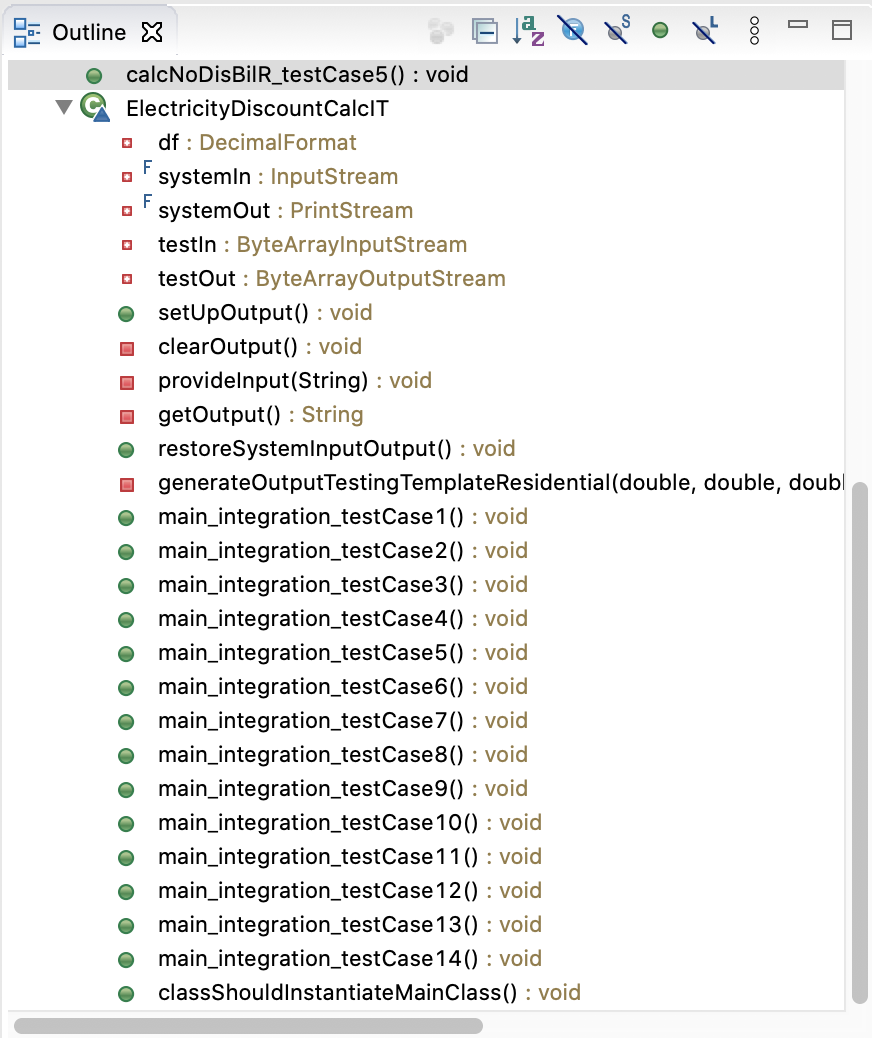
\includegraphics[width=\linewidth]{coverage/opti/14testcases.png}
			\caption{Modified test script}
        \end{subfigure}
		\label{fig:coveragereportinstance}
    \end{figure}

    \bigskip

    Now we can do a coverage report on eclipse

    \begin{figure}[h!]
		\centering
		\begin{subfigure}[b]{0.4\linewidth}
			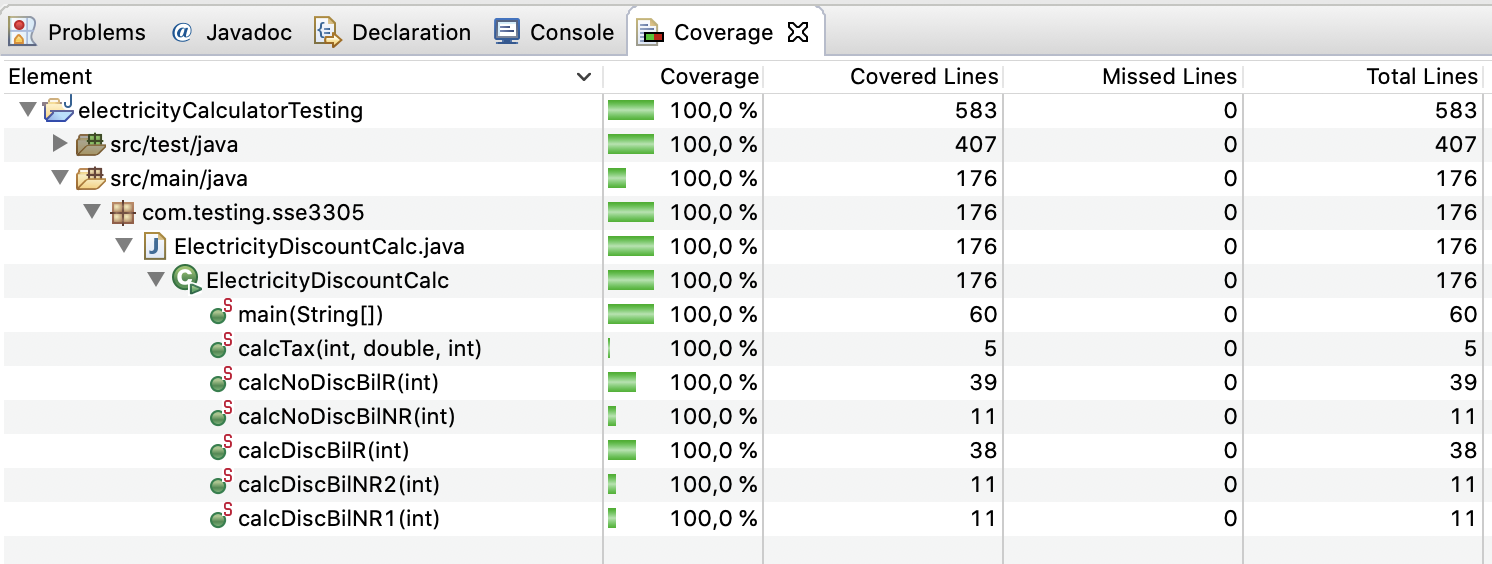
\includegraphics[width=\linewidth]{coverage/opti/line_coverage.png}
			\caption{Line coverage}
		\end{subfigure}
		\begin{subfigure}[b]{0.4\linewidth}
			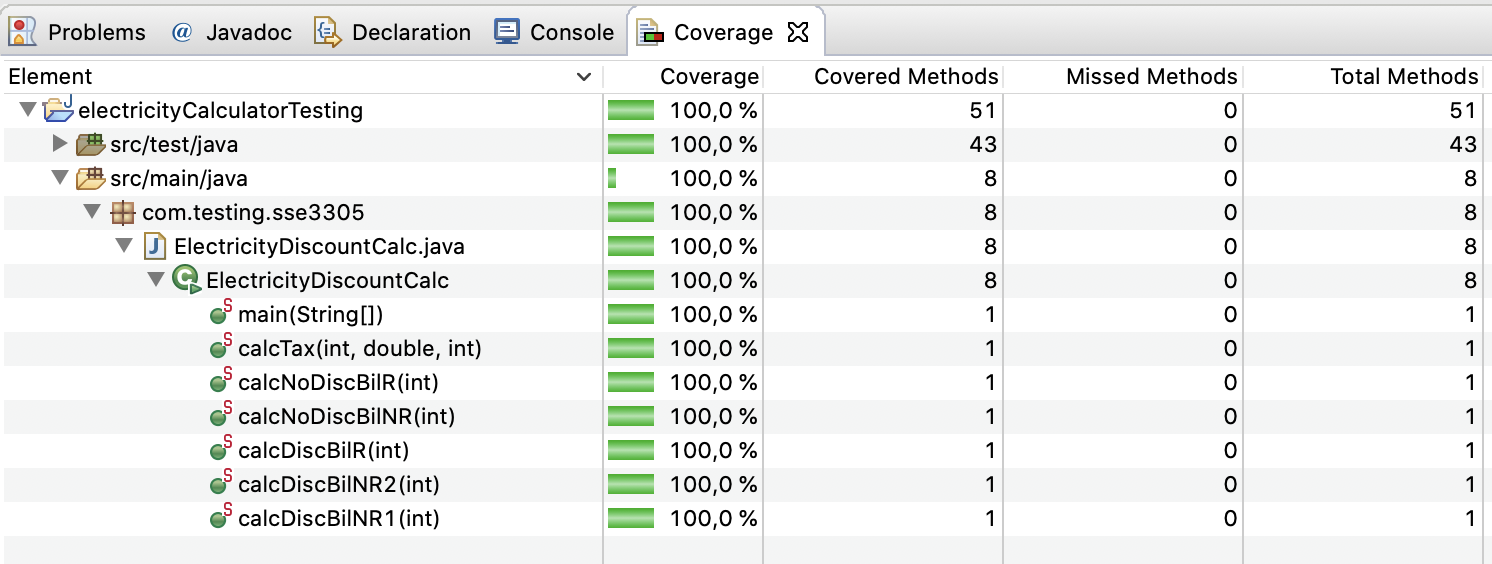
\includegraphics[width=\linewidth]{coverage/opti/method_coverage.png}
			\caption{Method coverage}
        \end{subfigure}
        \begin{subfigure}[b]{0.4\linewidth}
			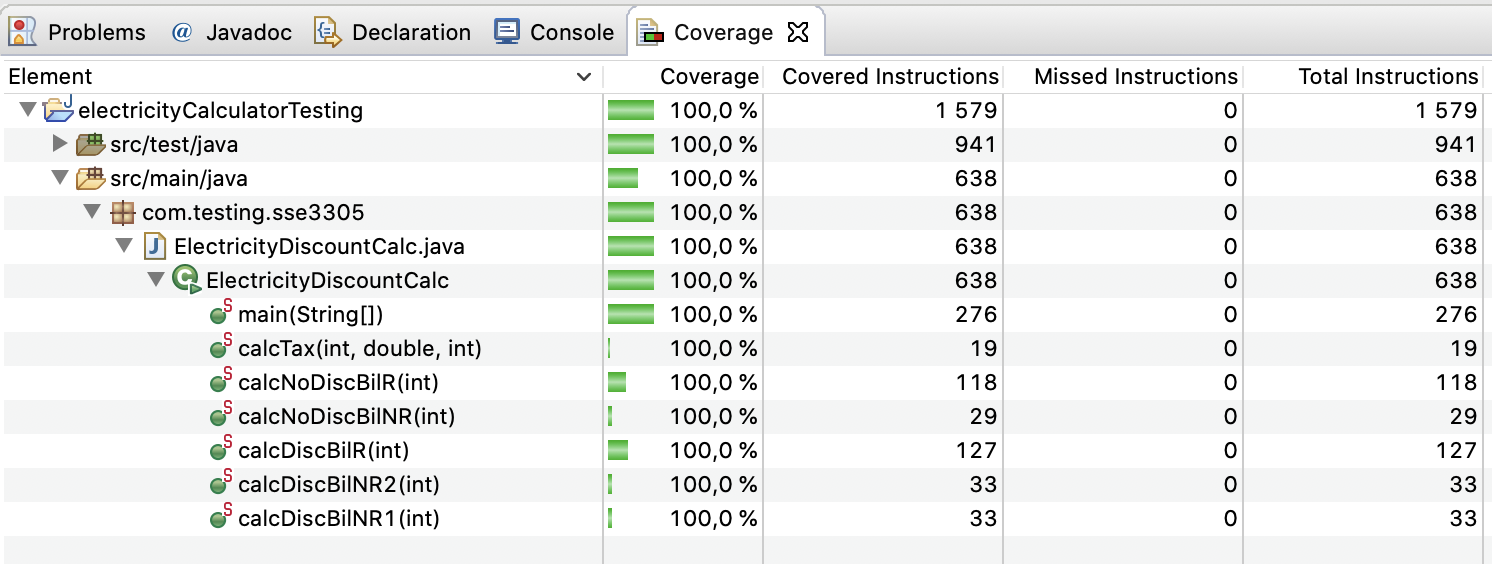
\includegraphics[width=\linewidth]{coverage/opti/instruction_coverage.png}
			\caption{Instruction coverage}
        \end{subfigure}
        \begin{subfigure}[b]{0.4\linewidth}
			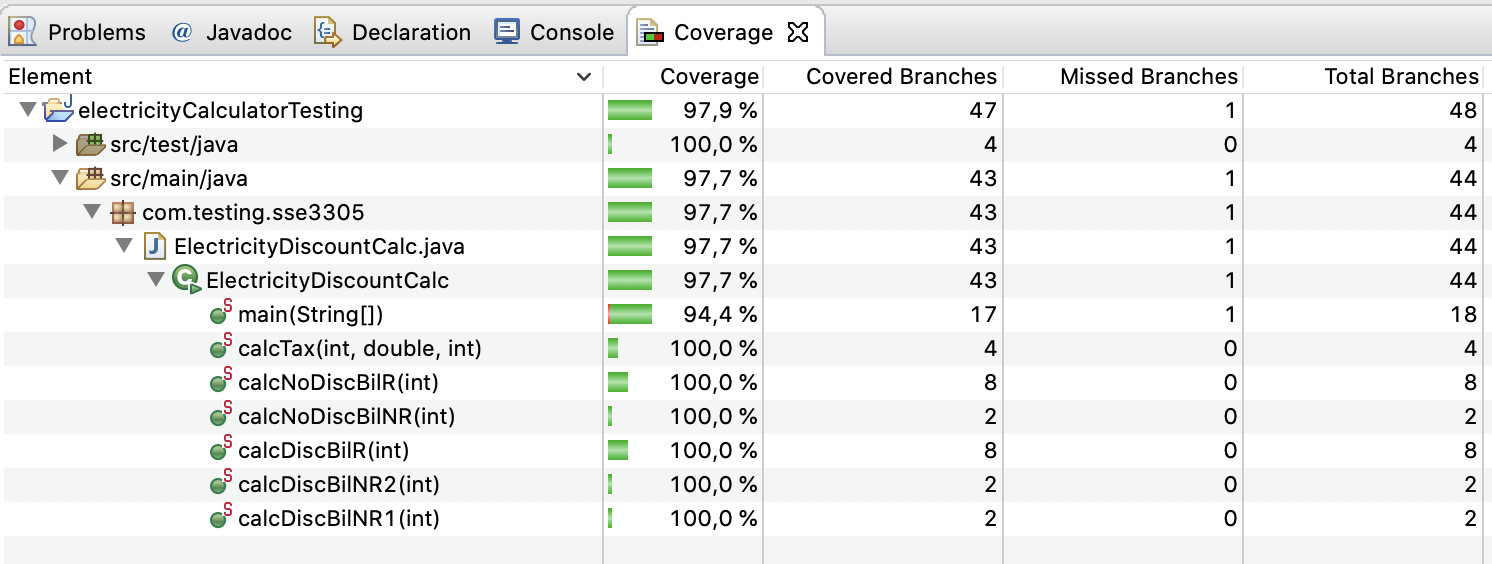
\includegraphics[width=\linewidth]{coverage/opti/branch_coverage.png}
			\caption{Branch coverage}
		\end{subfigure}
		\caption{Test coverage report with optimisation from Jacoco Eclipse}
		\label{fig:newcoveragereport}
	\end{figure}

    \bigskip

    As you can see on Figure ~\ref{fig:newcoveragereport}, except for the branch coverage, we succesfully increased the coverage percentage to 100\%.

    \bigskip

    Note: see \underline{\textbf{\textit{integration\_test\_script\_full.pdf}}} for more information

    \section{Conclusion}

    We saw in this report my strategy to test an electricity discount calculator software. 
    
    First of all, in terms of strategy and techniques, I can justify that the suggested solution is the most effective in testing: Basic Path Testing has been
    really efficient in term of coverage to perform the unit tests. Therefore, we are sure that any functions in the software can be used individually.

    Then, thanks to the decision table and the Bundary Value Analysis, the integration tests has covered the main part of the program.
    Even if there is still one branch that has not been covered by the tests, we can still guarranty the effectiveness of the software. 
    
    In addition, the coverage report justify and support the testing solution: we can consider a coverage very successfull hover 99\% which is the case here.

    Finally, Concerning the readiness of the system for deployment, we can assure that the software is ready to use and can be deployed to the users without having doubts on it
    performances. 
    
    The bottom line is that for further improvements, we are sure that the current code will not be affected by the new changes with this testing solution.
 
\end{document}